\documentclass[11pt,a4paper]{article}
\usepackage[margin=2.1cm]{geometry}
\usepackage{amsmath,booktabs,tabularx,xcolor,hyperref,enumitem,graphicx,float}
\hypersetup{colorlinks,linkcolor=blue!50!black,urlcolor=blue!50!black}
\setlist{itemsep=1pt,topsep=2pt}
\newcommand{\code}[1]{\texttt{\small #1}}
\definecolor{bad}{HTML}{B5403A}\definecolor{good}{HTML}{2E7D4F}

\title{Relative value: four pairs\\[2pt]\large CRWV against ORCL, HCA against THC, CCL against NCLH, MGM against WYNN}
\author{FundamentalQuantmental, HY Analyst}
\date{Bond prices to 17 September 2026; filings as known on 18 September 2026}

\begin{document}
\maketitle

\noindent\fcolorbox{gray}{gray!6}{\parbox{\dimexpr\linewidth-2\fboxsep-2\fboxrule}{%
\textbf{The four results, one line each}
\begin{enumerate}
\item \textbf{CRWV against ORCL:} CRWV pays 739 bp at 5 years against 136 bp. It pays more spread per unit of all four risk measures. The model leans long CRWV, but the model cannot see the renewal risk well. Treat it as a question, not a trade.
\item \textbf{HCA against THC:} THC pays 123 bp against 68 bp for almost the same leverage (3.1x against 2.9x). THC is the cheaper of the two. The gap closes fast (half-life about 5 weeks).
\item \textbf{CCL against NCLH:} both sit at the same distance above the fair line. Gap 3 bp. No trade.
\item \textbf{MGM against WYNN:} both sit below the fair line by a similar amount. Gap 13 bp. No trade worth the cost.
\end{enumerate}
\textbf{How far to trust this.} The fair line uses 8 issuers and one risk measure. It ranks; it does not price. Default loss is not in the alpha yet, because no current ratings are on file.}}

\section{How the report works, in four steps}
\begin{enumerate}
\item \textbf{Measure each issuer from its filing.} Lease-adjusted leverage $=(\text{debt}+\text{lease liabilities})/(\text{EBITDA}+\text{rent})$ (framework F5). Add the clock measures of Section 4.7 when the filer discloses signed revenue (RPO).
\item \textbf{Read each bond's spread from TRACE.} Volume-weighted yield of trades of \$100k or more over the last 10 days, minus the Treasury yield at the same maturity. Compare senior unsecured bonds with senior unsecured bonds.
\item \textbf{Compare the pair at the same maturity.} Fit each issuer's spread curve. Read both at 5 years. Divide spread by each risk measure: more spread per unit of risk is cheaper (Section 7.4).
\item \textbf{Place both on one fair line, then measure the speed of convergence.} Fit $\log s_{5y}=a+b\,\text{leverage}$ across all 8 issuers. The residual says who is cheap. TRACE history gives how fast the pair gap closes (Section 7.5).
\end{enumerate}

\section{The fair line across all eight issuers}
$\log s_{5y} = -5.64 + 0.312\times\text{lease-adjusted leverage}$ ($n=8$; the sign is correct). One more turn of leverage adds about 37\% to the spread.

\begin{center}
\begin{tabular}{@{}lrrrrl@{}}\toprule
Issuer & Leverage & 5y spread (bp) & Fair (bp) & Residual & Reading \\\midrule
CRWV & 8.9x & 739 & 574 & +0.25 & Cheap on leverage alone \\
ORCL & 4.3x & 137 & 135 & +0.01 & On the line \\
HCA & 2.9x & 68 & 88 & $-0.26$ & Rich \\
THC & 3.1x & 123 & 94 & +0.28 & Cheap \\
CCL & 3.5x & 129 & 105 & +0.21 & Cheap \\
NCLH & 5.7x & 258 & 208 & +0.22 & Cheap \\
MGM & 6.4x & 175 & 258 & $-0.39$ & Rich \\
WYNN & 6.0x & 165 & 226 & $-0.31$ & Rich \\\bottomrule
\end{tabular}
\end{center}
\textbf{What the table teaches.} The two casino names sit far below the line. Their leverage is high only because their landlord leases count as debt. The market does not price those leases as debt. That is a framework question (F5 lease rules for archetype A7), not a mispricing.

\newpage
\section{CRWV against ORCL}
\begin{figure}[H]\centering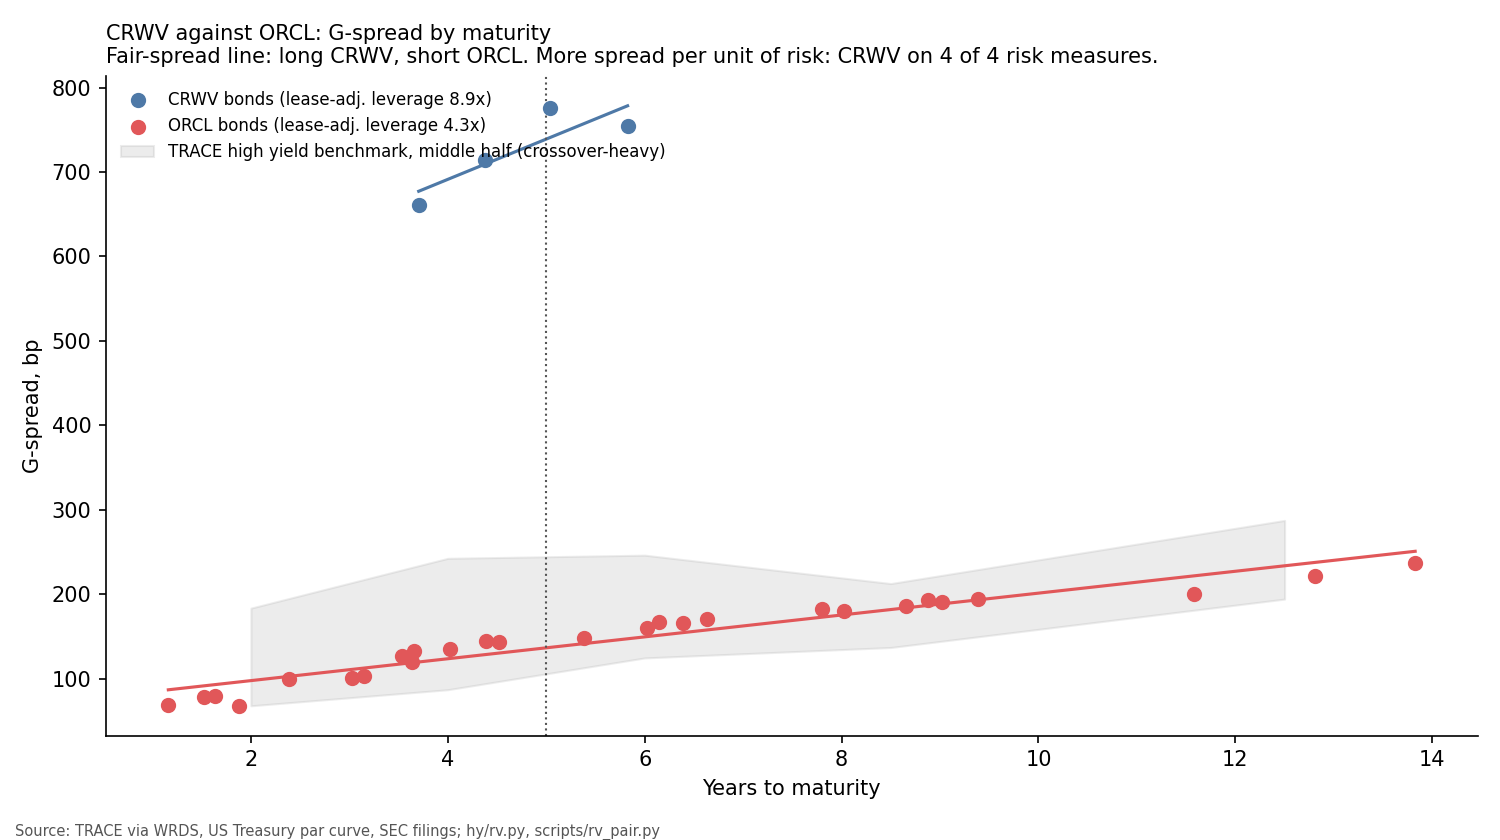
\includegraphics[width=\linewidth]{figures/rv_CRWV_ORCL.png}\end{figure}
\begin{center}
\begin{tabular}{@{}lrrl@{}}\toprule
Risk measure & CRWV & ORCL & bp per unit: CRWV against ORCL \\\midrule
Lease-adjusted leverage & 8.9x & 4.3x & 83 against 32 \\
Years of EBITDA that depend on renewal & 8.7 & 6.0 & 85 against 23 \\
Breakeven margin & 1.03 & 0.83 & 721 against 165 \\
Duration gap (years) & 2.9 & 4.9 & 257 against 28 \\\bottomrule
\end{tabular}
\end{center}
CRWV pays more per unit of every measure. On the fair line it is 159 bp cheap. The gap between the two names closes slowly: half-life 17 weeks. The convergence alpha is 388 bp of price over 6 months. \textbf{Do not act on that number.} The line knows only leverage. CRWV's renewal risk and its 72\% customer concentration are not on the line, and spread is convex in risk, so ``per unit'' flatters the riskier name. The gate of framework F9 fails: there is no dated catalyst, and the default-loss row is empty.

\section{HCA against THC}
\begin{figure}[H]\centering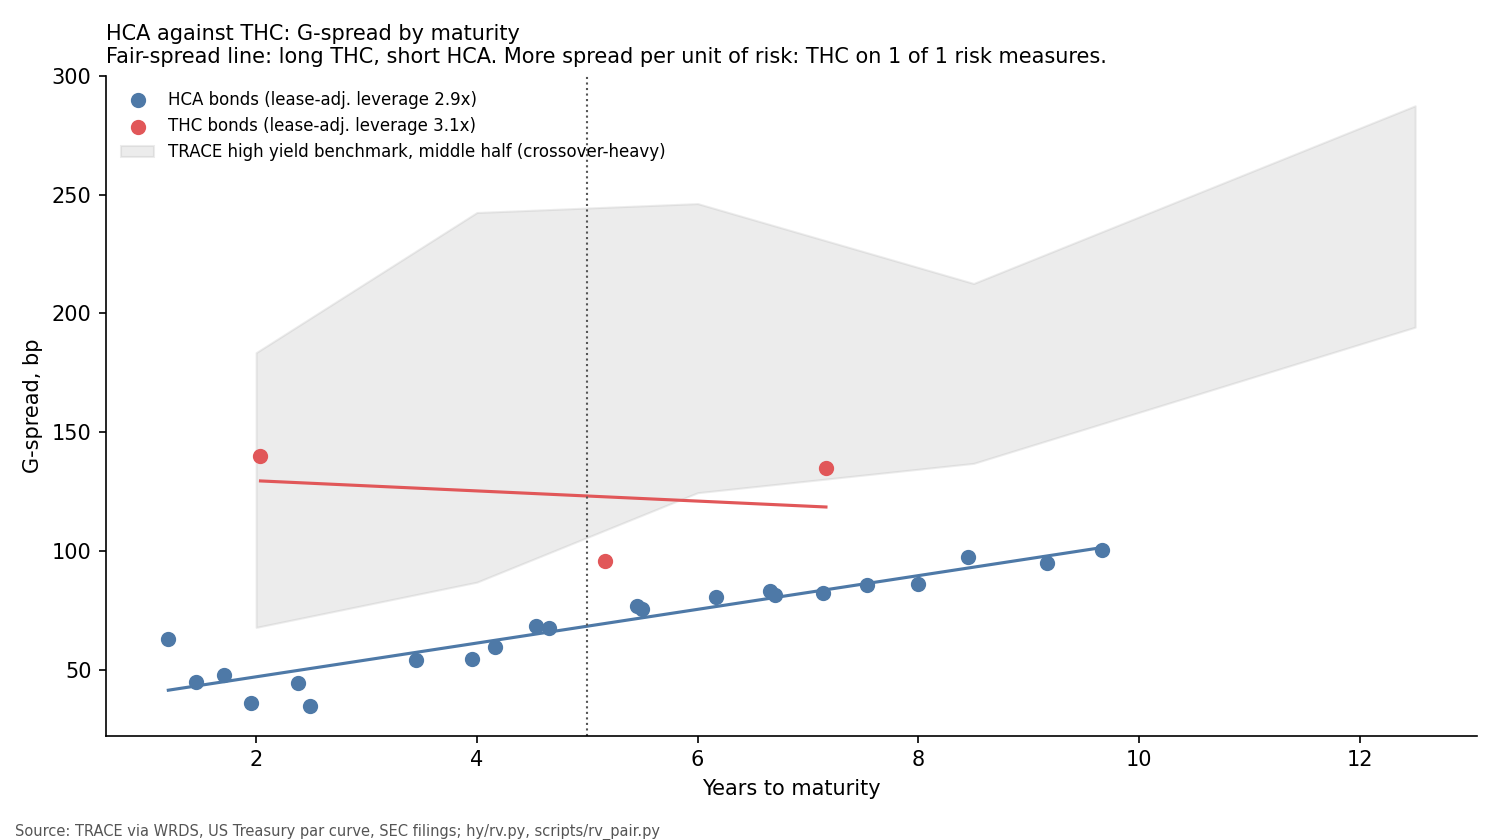
\includegraphics[width=\linewidth]{figures/rv_HCA_THC.png}\end{figure}
Same industry, same leverage (2.9x against 3.1x), and THC pays 55 bp more at 5 years. The book compares the same two names on margin (HCA 17.3\% against Tenet 5.9\%, p. 413); the margin gap is a reason for some of the spread gap. The pair gap closes with a half-life of about 5 weeks. Convergence alpha: 214 bp of price over 6 months, DV01-neutral at 5 years, before default loss and cost. Next check: add EBITDA margin and coverage to the fair line, then see if THC stays cheap.

\newpage
\section{CCL against NCLH}
\begin{figure}[H]\centering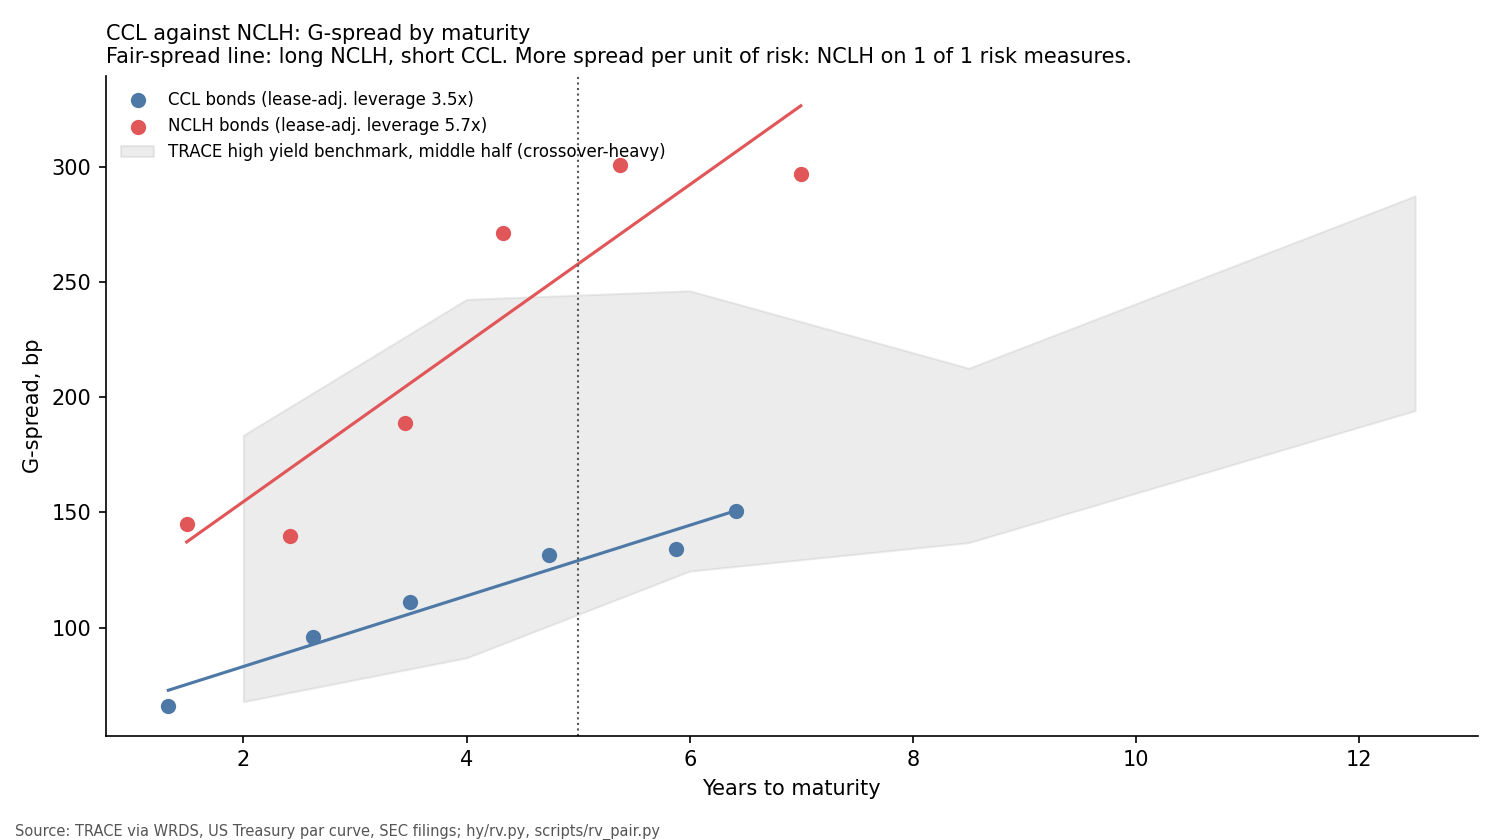
\includegraphics[width=\linewidth]{figures/rv_CCL_NCLH.png}\end{figure}
NCLH pays 258 bp against 129 bp, for 5.7x leverage against 3.5x. Both sit about the same distance above the fair line, so the pair gap is 3 bp. The market prices the leverage difference about as the line does. No trade.

\section{MGM against WYNN}
\begin{figure}[H]\centering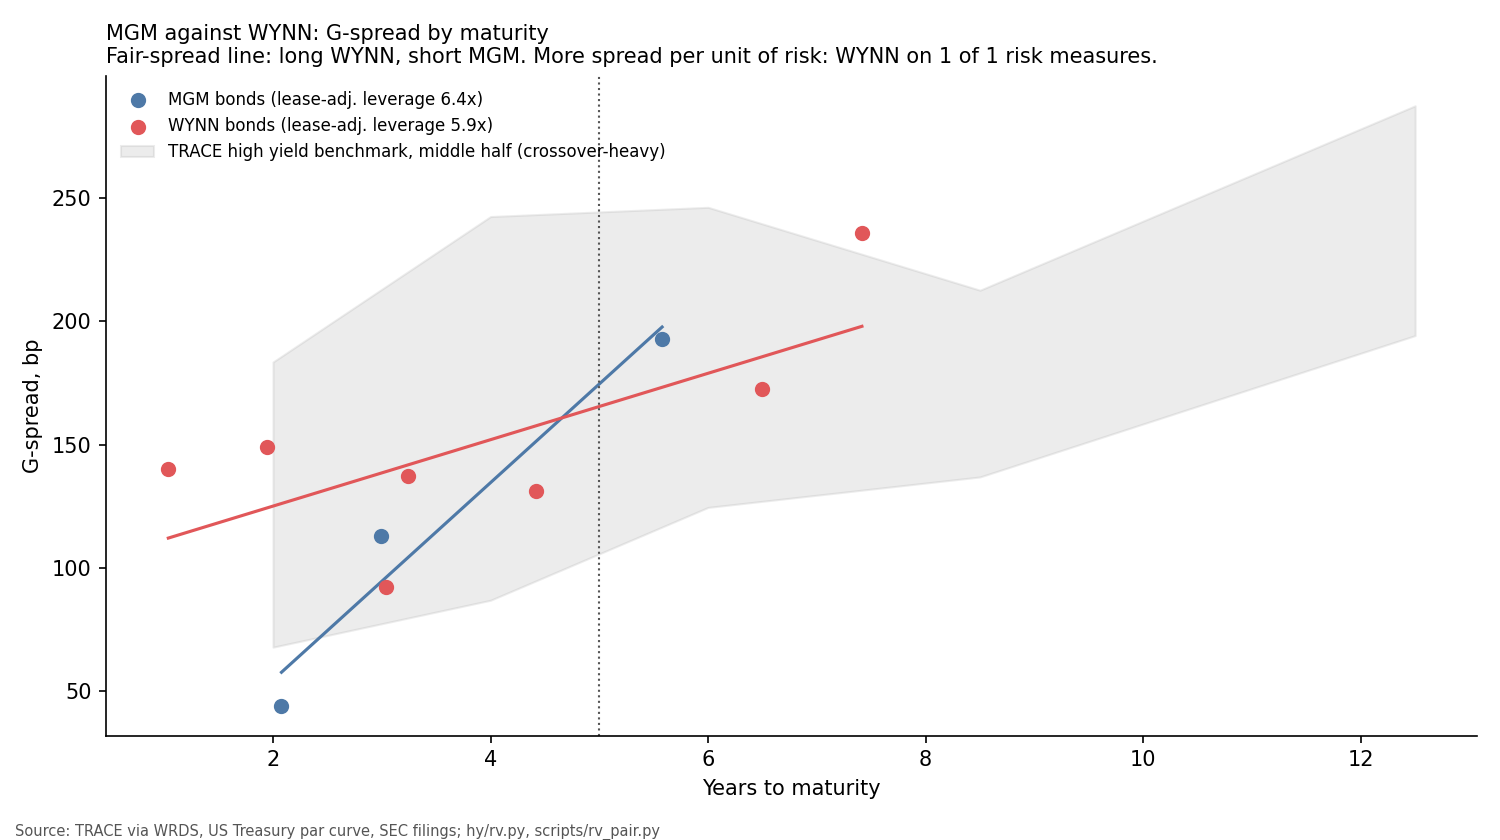
\includegraphics[width=\linewidth]{figures/rv_MGM_WYNN.png}\end{figure}
Both names are rich on the line for the lease reason above. WYNN is slightly cheaper than MGM: 13 bp at 5 years, gap half-life about 2 weeks, convergence alpha 54 bp of price over 6 months before cost. A round trip in two high yield bonds costs about that much. No trade.

\newpage
\section{What these numbers are not}
\begin{enumerate}
\item \textbf{Not net of default loss.} Default loss needs a default probability, which needs a rating. No current rating is on file. Fill \code{rating} in \code{data/analyst\_inputs/<ticker>.yaml}.
\item \textbf{Not net of cost.} The bid-ask round trip comes next.
\item \textbf{Not a fair-spread model.} Eight names and one factor. The full Section 7.2 model needs the whole universe.
\item \textbf{The TRACE benchmark is too tight.} FINRA's high yield flag includes crossover names. Use it as a shape, not a level.
\item \textbf{Two inputs use a fallback.} THC and MGM each lost one quarter of EBITDA to the XBRL definition check; their LTM EBITDA is three quarters times 4/3.
\end{enumerate}

\section{How to test the alpha forecast}
The test asks one question: when the model predicts 100 bp of alpha, does the bond earn about 100 bp more than its hedge? Five steps.
\begin{enumerate}
\item \textbf{Replay history with no look-ahead.} Every Friday from 2008 to 2026, rebuild the prediction using only data with \code{available\_at} before that Friday: Compustat point-in-time, filing dates from EDGAR, TRACE prices, forecast vintages (SPF and SEP archives go back decades). Keep bonds that later default, priced at recovery.
\item \textbf{Measure what the bond actually earned.} Over each horizon: price change plus coupon, minus the Treasury hedge at the same duration, minus the high yield index move times the bond's beta. That is the realised alpha.
\item \textbf{Score the ranking.} Rank correlation (IC) between predicted and realised alpha on each date. Correct the t-statistic for overlapping horizons. The project's own bar: positive after cost in at least three of the four cycles 2008, 2015, 2020, 2022.
\item \textbf{Score the size.} Sort into ten buckets by predicted alpha. Regress realised on predicted: the slope should be near 1 and the intercept near 0. A slope of 0.3 means the model is right about direction but three times too confident.
\item \textbf{Score each part on its own.} Carry against realised carry. Convergence: does the gap close at the predicted half-life out of sample? Loss: realised default rate against the predicted default probability by bucket. Spread of outcomes: the realised alpha against the predicted mean plus or minus \code{alpha\_sd} should look uniform (the same PIT test the leverage forecast already passes).
\end{enumerate}
\textbf{The benchmark that matters.} Run the same test on the simplest rule: buy the widest bonds. The model earns its keep only if it beats that rule after cost.

\end{document}
